\documentclass{article}
\usepackage[utf8]{inputenc}
\usepackage[T1]{fontenc}
\usepackage[french]{babel}
\usepackage{amsmath}
\usepackage{amssymb}
\usepackage{graphicx}
\usepackage{booktabs}

\begin{document}

\section{Projet : VNF Chain Optimization}

Ce notebook formalise la logique et la modélisation mathématique pour résoudre le projet d'optimisation (placements de VNF sur des serveurs).

\subsection{Objectif Global}
Trouver un placement optimal de $n$ fonctions réseau virtuelles (VNF) sur $m$ serveurs physiques qui minimise la charge maximale parmi tous les serveurs (le goulot d'étranglement ou \textbf{cycle time} $CT$), tout en respectant les contraintes de précédence entre les VNF.

\vspace{1em}
\hrule
\vspace{1em}

\section{Phase 1 : Solution Exacte (MILP)}

Cette phase formalise le problème comme un programme linéaire en nombres entiers (MILP) et utilise Gurobi pour trouver la solution optimale.

\subsection{1. Formulation Mathématique}

\subsubsection{1.1 Variables de Décision}

\begin{itemize}
    \item $x_{jk} \in \{0, 1\}$ : Vaut 1 si la VNF $j$ est placée sur le serveur $k$, 0 sinon.
    \item $s_j \in \{1, \dots, m\}$ : Indice du serveur sur lequel la VNF $j$ est placée.
    \item $CT \ge 0$ : Le "Cycle Time" ou latence du goulot d'étranglement (charge maximale d'un serveur).
\end{itemize}

\subsubsection{1.2 Fonction Objectif}

Minimiser $CT$

\subsubsection{1.3 Contraintes}

\begin{enumerate}
    \item \textbf{Unicité du placement} : Chaque VNF $j$ doit être placée sur exactement un serveur.
    \[\sum_{k=1}^m x_{jk} = 1 \quad \forall j \in J\]

    \item \textbf{Définition de l'indice du serveur} : Lien entre les variables binaires $x$ et l'indice $s_j$.
    \[s_j = \sum_{k=1}^m k \cdot x_{jk} \quad \forall j \in J\]

    \item \textbf{Respect des précédences} : Pour chaque arc $(i, j) \in P$, la VNF $i$ doit être placée sur le même serveur ou un serveur précédent par rapport à $j$.
    \[s_i \le s_j \quad \forall (i, j) \in P\]

    \item \textbf{Goulot d'étranglement} : La somme des temps de traitement sur n'importe quel serveur $k$ ne doit pas dépasser le cycle time.
    \[\sum_{j=1}^n t_j \cdot x_{jk} \le CT \quad \forall k \in K\]
\end{enumerate}

\subsection{2. Résultats et Analyse}

\subsubsection{2.1 Tableau des résultats}

Le tableau suivant regroupe les résultats de notre modèle MILP sur les 24 instances du benchmark SALBPGen. Le nombre de serveurs $m$ est spécifique à chaque instance (issu du benchmark). Une limite de temps de 30 minutes par instance a été imposée.

\begin{table}[h!]
\centering
\small
\begin{tabular}{l c c c c c c c}
\toprule
\textbf{Instance} & $\boldsymbol{n}$ & $\boldsymbol{m}$ & \textbf{OS} & \textbf{Préc.} & \textbf{$\sum t_j$} & $\boldsymbol{CT^*}$ & \textbf{Temps (s)} \\
\midrule
n=20\_1  & 20 & 3  & 0.268 & 16 & 2882  & 962  & 0.054 \\
n=20\_2  & 20 & 3  & 0.300 & 19 & 2861  & 954  & 0.007 \\
n=20\_3  & 20 & 3  & 0.300 & 18 & 2785  & 930  & 0.056 \\
n=20\_4  & 20 & 3  & 0.289 & 18 & 2727  & 909  & 0.036 \\
n=20\_5  & 20 & 3  & 0.289 & 18 & 2837  & 950  & 0.076 \\
n=20\_6  & 20 & 3  & 0.295 & 19 & 2914  & 973  & 0.045 \\
n=20\_7  & 20 & 3  & 0.300 & 18 & 2786  & 930  & 0.041 \\
n=20\_8  & 20 & 3  & 0.289 & 20 & 2985  & 996  & 0.071 \\
n=20\_9  & 20 & 3  & 0.289 & 18 & 2925  & 976  & 0.055 \\
n=20\_10 & 20 & 3  & 0.279 & 17 & 2831  & 945  & 0.067 \\
n=20\_11 & 20 & 3  & 0.279 & 18 & 2766  & 924  & 0.089 \\
n=20\_12 & 20 & 3  & 0.300 & 17 & 2930  & 977  & 0.023 \\
n=20\_13 & 20 & 3  & 0.268 & 17 & 2896  & 967  & 0.078 \\
n=20\_14 & 20 & 3  & 0.263 & 17 & 2979  & 994  & 0.086 \\
n=20\_15 & 20 & 3  & 0.295 & 18 & 2981  & 994  & 0.037 \\
n=20\_16 & 20 & 12 & 0.232 & 17 & 10376 & 981  & 0.751 \\
n=20\_17 & 20 & 10 & 0.295 & 17 & 9134  & 969  & 0.366 \\
n=20\_18 & 20 & 11 & 0.300 & 20 & 9524  & 960  & 0.191 \\
n=20\_19 & 20 & 14 & 0.268 & 18 & 11113 & 1000 & 0.240 \\
n=20\_20 & 20 & 11 & 0.295 & 17 & 9829  & 1000 & 0.298 \\
\midrule
n=50\_1  & 50 & 8  & 0.196 & 58 & 7276  & 910  & 11.52 \\
n=50\_2  & 50 & 6  & 0.195 & 56 & 5585  & 931  & 1.49  \\
\midrule
n=100\_1 & 100 & 23 & 0.196 & 105 & 22723 & N/A$^\dagger$ & $>$1800 \\
n=100\_2 & 100 & 21 & 0.195 & 104 & 20262 & N/A$^\dagger$ & $>$89  \\
\bottomrule
\end{tabular}
\caption{Résultats complets de l'optimisation MILP (Phase 1). $^\dagger$Instances n'ayant pas convergé dans la limite de 30 minutes.}
\label{tab:results}
\end{table}

\subsubsection{2.2 Analyse graphique des performances}

La figure \ref{fig:resol_time} illustre l'évolution du temps de résolution en fonction de la taille de l'instance et de l'Order Strength.

\begin{figure}[h!]
    \centering
    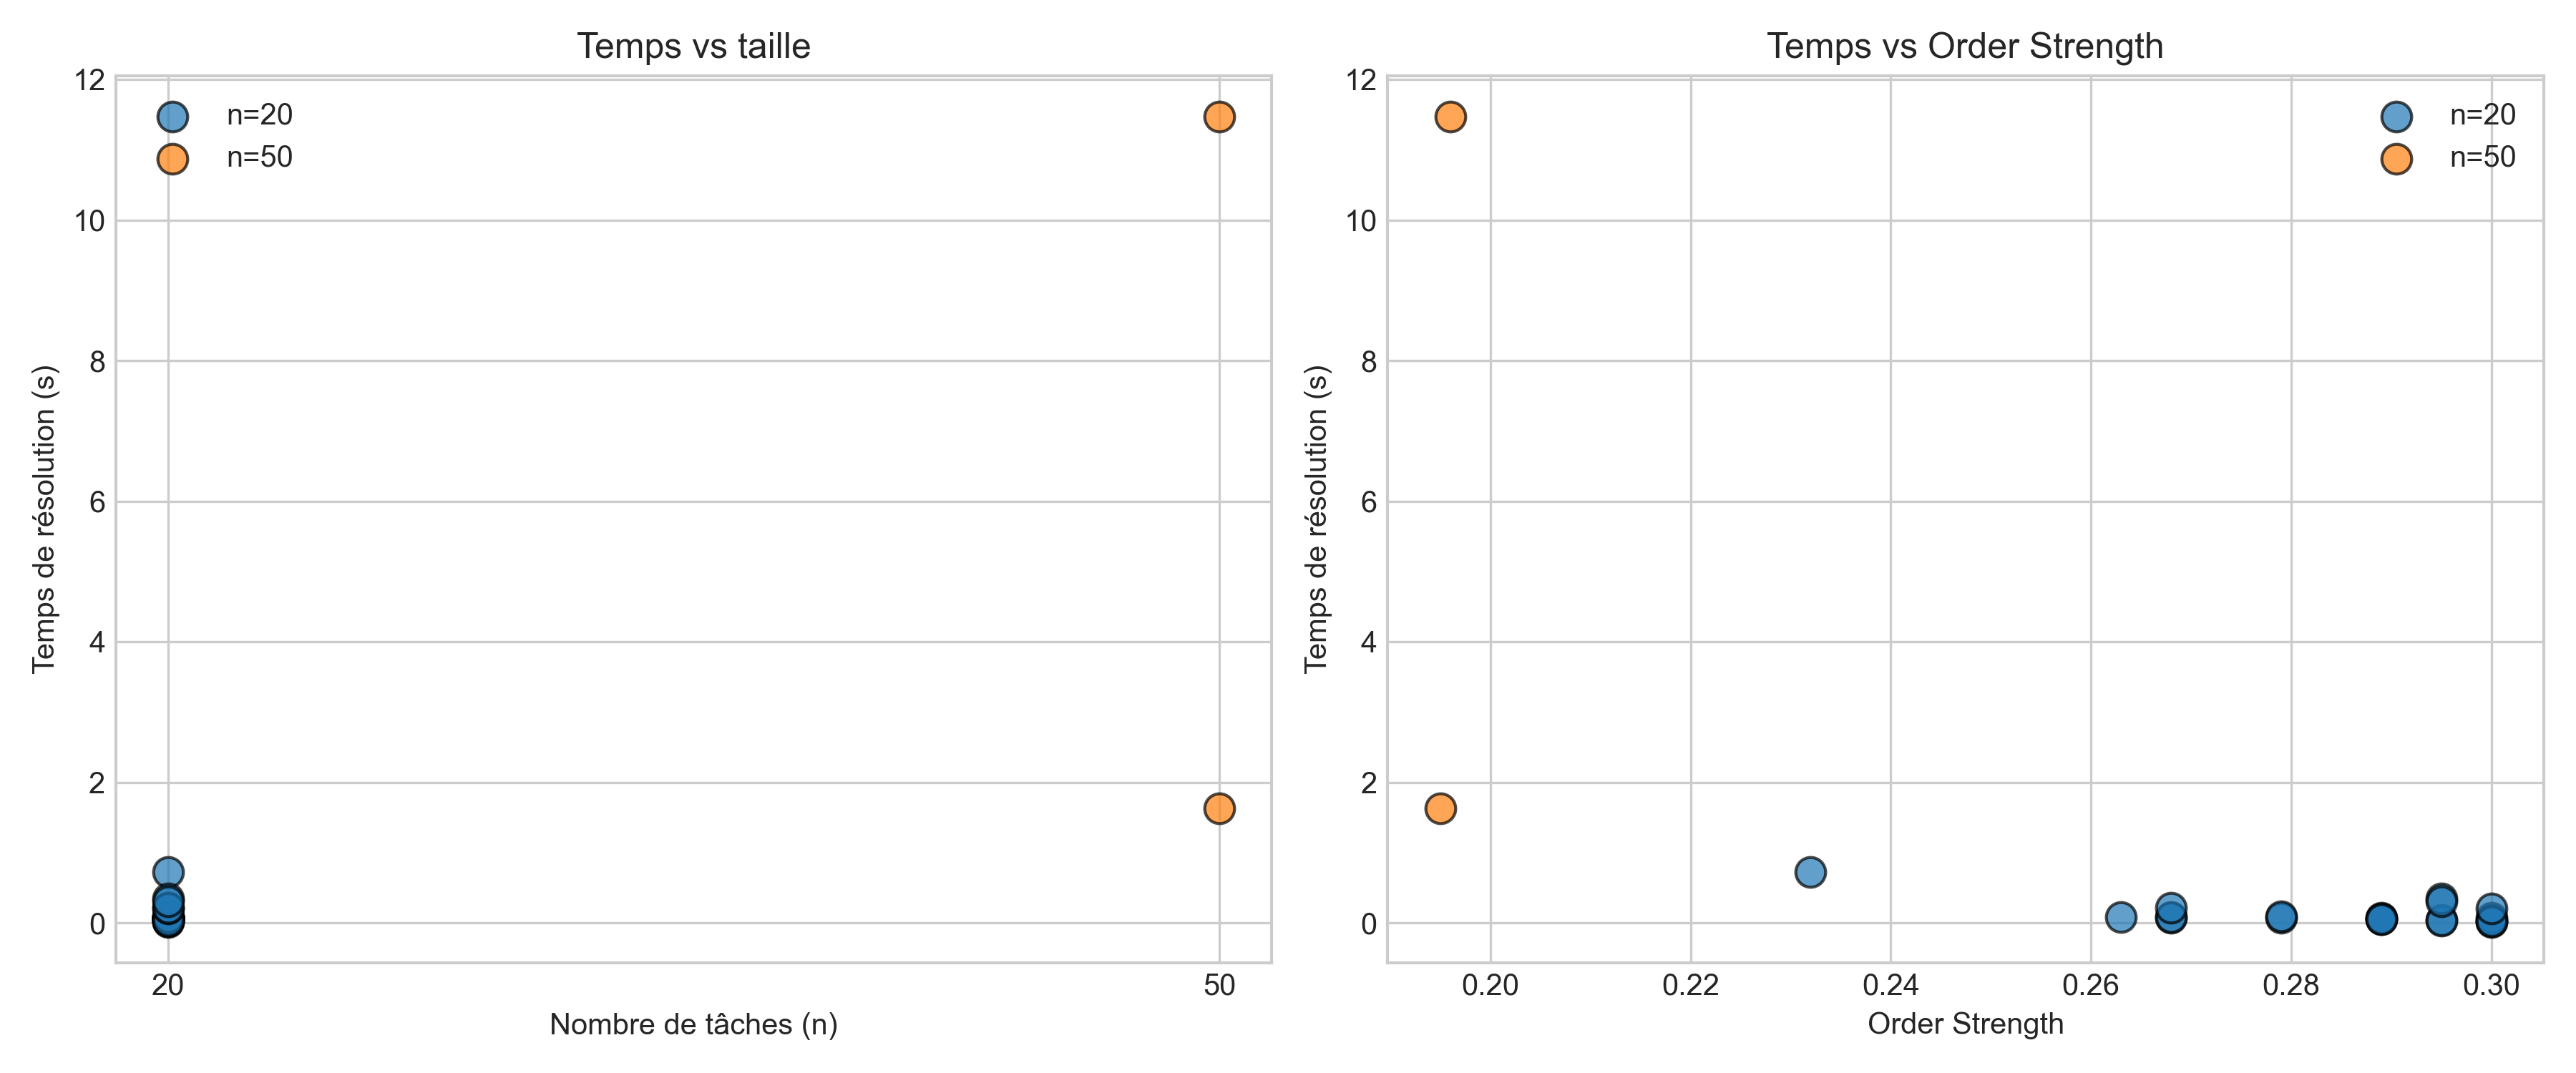
\includegraphics[width=\textwidth]{resol_time_analysis.png}
    \caption{Temps de résolution en fonction de la taille du problème ($n$) et de l'Order Strength (OS).}
    \label{fig:resol_time}
\end{figure}

\subsection{Conclusions}
\begin{itemize}
    \item \textbf{Instances $n=20$} : Toutes les 20 instances sont résolues à l'optimalité en moins d'une seconde ($\leq 0.75$s). Les $CT^*$ obtenus respectent la borne $CT \leq 1000$ imposée par le benchmark. Les instances 1--15 ($m=3$) sont les plus rapides ; les instances 16--20 ($m \geq 10$), plus coûteuses en nombre de variables binaires, restent néanmoins résolues très efficacement.
    \item \textbf{Instances $n=50$} : Résolues à l'optimalité en 1.5s à 11.5s. L'augmentation significative du temps pour n=50\_1 ($m=8$) par rapport à n=50\_2 ($m=6$) illustre l'impact du nombre de serveurs sur la combinatoire ($n \times m$ variables binaires).
    \item \textbf{Instances $n=100$} : Non résolues dans la limite de 30 minutes. Avec $m \geq 21$ serveurs, le modèle comporte plus de $n \times m = 2100$ variables binaires, rendant l'exploration du Branch-and-Bound très coûteuse. Cela motive le recours aux heuristiques (Phase 2).
    \item \textbf{Impact de $m$ vs.\ $n$} : Le facteur déterminant pour la difficulté n'est pas uniquement $n$ mais le produit $n \times m$, qui détermine le nombre de variables binaires $x_{jk}$.
\end{itemize}

\section{Phase 3 : Placement de VNF avec Prise en Compte de l'Énergie (EVNF-P)}

\subsection{1. Motivation Énergétique et Contexte NFV}

Les centres de données représentent environ 1--2\% de la consommation mondiale d'électricité, et cette part augmente avec le déploiement de la 5G et de l'edge computing. Un problème opérationnel critique est celui des \textbf{points chauds thermiques} : lorsqu'un serveur concentre des VNFs énergivores, la température de son CPU augmente fortement, ce qui :
\begin{itemize}
    \item dégrade les performances (throttling),
    \item réduit la durée de vie du matériel,
    \item déclenche des réponses de refroidissement coûteuses.
\end{itemize}

Les opérateurs de centres de données estiment que le refroidissement à lui seul représente \textbf{30--40\% de la dépense énergétique totale}. Un mauvais équilibrage du placement des VNF est un facteur direct de cette surconsommation.

Cela crée une forte incitation à intégrer directement des critères énergétiques dans la décision de placement : minimiser le pic de stress énergétique des serveurs (plutôt que seulement la latence) garantit qu'aucun serveur unique ne supporte une part disproportionnée de la charge énergétique, permettant un refroidissement plus uniforme et améliorant la durée de vie globale de l'infrastructure.

\subsection{2. Formulation du Modèle EVNF-P}

\subsubsection{2.1 Intensité Énergétique des VNF}

Toutes les VNFs ne consomment pas la même puissance par unité de charge de traitement. On caractérise chaque VNF $j \in J$ par un \textbf{score d'intensité énergétique} fixe $e_j \in \{1, \ldots, 15\}$, représentant sa consommation d'énergie normalisée par unité de charge CPU.

\begin{table}[h!]
\centering
\small
\begin{tabular}{c c l l}
\toprule
\textbf{Score $e_j$} & \textbf{Niveau} & \textbf{Types typiques de VNF} & \textbf{Action requise} \\
\midrule
1 & Négligeable & ACL simple, routage statique & Aucune \\
2--4 & Faible & NAT, répartiteur L4 basique & Surveiller \\
5--8 & Moyen & Pare-feu avec états, IDS & Planifier la capacité \\
9--12 & Élevé & Terminaison TLS, DPI & Éviter la concentration \\
13--15 & Très élevé & Détection ML, transcodage vCDN & Répartir en urgence \\
\bottomrule
\end{tabular}
\caption{Classification des scores d'intensité énergétique pour les VNF.}
\end{table}

Pour le benchmark, les scores $e_j$ sont générés uniformément dans $\{1, \ldots, 15\}$ avec la graine aléatoire fixe \texttt{seed=42}.

\subsubsection{2.2 Stress Énergétique Pondéré par la Charge}

Une fois les VNFs placées sur les serveurs, il faut un nombre unique pour représenter le stress énergétique de chaque serveur. L'approche naïve (somme des scores $\sum_j e_j x_{jk}$) est trompeuse car elle ignore combien de temps chaque VNF fonctionne réellement.

\textbf{Exemple illustratif.} Le serveur $k$ héberge deux VNFs :
\begin{itemize}
    \item VNF-A : charge $t_A = 2\,\mu\text{s}$, score $e_A = 12$ (DPI rare)
    \item VNF-B : charge $t_B = 58\,\mu\text{s}$, score $e_B = 2$ (NAT fréquent)
\end{itemize}
La somme naïve donne $12 + 2 = 14$, suggérant un stress maximal. Or VNF-A ne représente que 3\% du temps de traitement ; le stress réaliste est dominé par VNF-B (faible intensité).

On adopte donc un \textbf{score énergétique moyen pondéré par la charge} comme métrique du stress au niveau du serveur. Pour un serveur $k \in K$ :
\[
E_k = \frac{\sum_{j \in J} e_j \cdot t_j \cdot x_{jk}}{\sum_{j \in J} t_j \cdot x_{jk}} = \frac{N_k}{L_k}
\]
où $N_k$ est la charge de traitement pondérée par l'énergie et $L_k$ est la charge totale de traitement (définie en phase 1).

Pour l'exemple : $E_k = (12 \times 2 + 2 \times 58) / 60 \approx 2.33$, reflétant fidèlement le faible stress énergétique global.

\subsubsection{2.3 Formulation MILP EVNF-P}

Étant donné une borne de latence goulot $\bar{C}$ (obtenue à partir de la phase 1, par exemple $\bar{C} = 1.05 \times CT^*$), le modèle EVNF-P minimise le pic de stress énergétique sous les contraintes de placement, précédence et latence :

\begin{align}
\min_{x, s, E_k, E_{\max}} \quad & E_{\max} \label{evnfp:obj} \\
\text{s.c.} \quad & \sum_{k \in K} x_{jk} = 1 \quad \forall j \in J \label{evnfp:assign} \\
& s_j = \sum_{k \in K} k \cdot x_{jk} \quad \forall j \in J \label{evnfp:server_idx} \\
& s_i \le s_j \quad \forall (i, j) \in P \label{evnfp:prec} \\
& L_k = \sum_{j \in J} t_j \cdot x_{jk} \quad \forall k \in K \label{evnfp:load} \\
& L_k \le \bar{C} \quad \forall k \in K \label{evnfp:latency_bound} \\
& E_k \cdot L_k = \sum_{j \in J} e_j \cdot t_j \cdot x_{jk} \quad \forall k \in K \quad \text{[non-linéaire]} \label{evnfp:energy} \\
& E_k \le E_{\max} \quad \forall k \in K \label{evnfp:energy_max} \\
& x_{jk} \in \{0, 1\}, \quad s_j \in \{1, \ldots, m\} \quad \forall j \in J, k \in K \label{evnfp:bin} \\
& L_k \ge 0, \quad E_{\min} \le E_k \le E_{\max}^{\text{bound}} \quad \forall k \in K \label{evnfp:bounds}
\end{align}

\textbf{Explication des contraintes :}
\begin{itemize}
    \item \eqref{evnfp:obj} : minimiser le pic de stress énergétique garantit qu'aucun serveur ne devient un goulot thermique.
    \item \eqref{evnfp:assign}--\eqref{evnfp:prec} : identiques à phase 1 (placement unique, précédence).
    \item \eqref{evnfp:load}--\eqref{evnfp:latency_bound} : charge et limite de latence (plutôt que de minimiser CT, on fixe C̄).
    \item \eqref{evnfp:energy} : définit le stress pondéré par la charge via le produit $E_k \cdot L_k = N_k$ (source de non-linéarité).
    \item \eqref{evnfp:energy_max} : lie chaque stress local au maximum global.
\end{itemize}

\subsection{3. Linéarisation via Inégalités de McCormick}

\subsubsection{3.1 Cas Bilinéaire : Variable Continue × Binaire}

La contrainte \eqref{evnfp:energy} introduit des termes bilinéaires $E_k \cdot x_{jk}$ (produit d'une variable continue et d'une variable binaire). C'est la source de la non-linéarité.

\textbf{L'observation clé} : lorsqu'un des deux facteurs est binaire, la relaxation de McCormick est \textbf{exacte}. Elle n'introduit aucune erreur d'approximation, et les quatre inégalités de McCormick caractérisent exactement le produit sur l'ensemble faisable entier.

\subsubsection{3.2 Dérivation des Quatre Inégalités de McCormick}

Soit $z_{jk} = E_k \cdot x_{jk}$ où $E_k$ est continue bornée par $E_{\min} \le E_k \le E_{\max}^{\text{bound}}$ et $x_{jk} \in \{0, 1\}$ est binaire.

L'enveloppe de McCormick fournit quatre inégalités :

\begin{align}
z_{jk} &\ge E_{\min} \cdot x_{jk} \label{mc:1} \\
z_{jk} &\ge E_k - E_{\max}^{\text{bound}} \cdot (1 - x_{jk}) \label{mc:2} \\
z_{jk} &\le E_{\max}^{\text{bound}} \cdot x_{jk} \label{mc:3} \\
z_{jk} &\le E_k - E_{\min} \cdot (1 - x_{jk}) \label{mc:4}
\end{align}

\textbf{Justification :}
\begin{itemize}
    \item Lorsque $x_{jk} = 0$, le produit doit être nul. Les inégalités \eqref{mc:1} et \eqref{mc:3} forcent $z_{jk} = 0$.
    \item Lorsque $x_{jk} = 1$, le produit doit être égal à $E_k$. Les inégalités \eqref{mc:2} et \eqref{mc:4} forcent $z_{jk} = E_k$.
    \item Ces quatre inégalités forment une \textbf{formulation MILP exacte} (pas d'approximation).
\end{itemize}

\subsubsection{3.3 Application à EVNF-P}

On introduit des variables auxiliaires $Z_{jk} = E_k \cdot x_{jk}$ et on remplace la contrainte \eqref{evnfp:energy} par :

\[
\sum_{j \in J} Z_{jk} = \sum_{j \in J} e_j \cdot t_j \cdot x_{jk} \quad \forall k \in K
\]

Plus 4 inégalités de McCormick pour chaque $(j, k)$, donnant une formulation MILP linéaire exacte avec $|J| \times |K|$ variables auxiliaires supplémentaires.

\subsection{4. Validation Numérique (Section 2.15)}

\subsubsection{4.1 Instance Illustrative : 8 VNF, 3 Serveurs}

Tableau des données d'entrée :

\begin{table}[h!]
\centering
\small
\begin{tabular}{c l c c}
\toprule
\textbf{VNF} & \textbf{Fonction} & $\boldsymbol{t_j}$ ($\mu\text{s}$) & $\boldsymbol{e_j}$ (score) \\
\midrule
1 & Pare-feu avec états (FW) & 8 & 7 \\
2 & Traduction d'adresses (NAT) & 10 & 3 \\
3 & Système de prévention (IPS) & 1 & 12 \\
4 & Inspection approfondie (DPI) & 9 & 10 \\
5 & Détection d'intrusion (IDS) & 9 & 5 \\
6 & Terminaison TLS & 3 & 14 \\
7 & Répartiteur de charge (LB) & 2 & 9 \\
8 & Contrôleur de trafic (TC) & 1 & 4 \\
\bottomrule
\end{tabular}
\caption{Instance illustrative : 8 VNF avec charges et scores énergétiques.}
\end{table}

DAG de précédence : $P = \{(1,3), (1,6), (2,4), (2,5), (3,7), (4,7), (5,7), (6,8), (7,8)\}$

\subsubsection{4.2 Cible A : Placement Optimal de Phase 1 (M1)}

Le modèle M1 (minimiser CT) donne le placement optimal avec $\bar{C} = 17$ :
\begin{align*}
S_1 &= \{\text{NAT}\}, \quad L_1 = 10 \\
S_2 &= \{\text{FW}, \text{DPI}\}, \quad L_2 = 8 + 9 = 17 \\
S_3 &= \{\text{IPS}, \text{IDS}, \text{TLS}, \text{LB}, \text{TC}\}, \quad L_3 = 1 + 9 + 3 + 2 + 1 = 16
\end{align*}

Stress énergétique pondéré :
\begin{align*}
E_1 &= \frac{10 \times 3}{10} = 3.0 \\
E_2 &= \frac{8 \times 7 + 9 \times 10}{17} = \frac{146}{17} \approx 8.5882 \\
E_3 &= \frac{1 \times 12 + 9 \times 5 + 3 \times 14 + 2 \times 9 + 1 \times 4}{16} = \frac{121}{16} \approx 7.5625
\end{align*}

\textbf{Résultat :} $E_{\max} = \max(3.0, 8.5882, 7.5625) \approx \boxed{8.5882}$

Le serveur $S_2$ constitue le point chaud thermique : il héberge le module DPI (très énergivore) en plus du FW lourd, conduisant à un score pondéré élevé.

\subsubsection{4.3 Cible B : Placement Optimal EVNF-P}

Le modèle EVNF-P (minimiser $E_{\max}$) avec $\bar{C} = 34$ donne le placement suivant :
\begin{align*}
S_1 &= \{\text{FW}\}, \quad L_1 = 8 \\
S_2 &= \{\text{NAT}, \text{IPS}, \text{DPI}, \text{IDS}, \text{TLS}, \text{LB}\}, \quad L_2 = 10 + 1 + 9 + 9 + 3 + 2 = 34 \\
S_3 &= \{\text{TC}\}, \quad L_3 = 1
\end{align*}

Stress énergétique pondéré :
\begin{align*}
E_1 &= \frac{8 \times 7}{8} = 7.0 \\
E_2 &= \frac{10 \times 3 + 1 \times 12 + 9 \times 10 + 9 \times 5 + 3 \times 14 + 2 \times 9}{34} = \frac{237}{34} \approx 6.9706 \\
E_3 &= \frac{1 \times 4}{1} = 4.0
\end{align*}

\textbf{Résultat :} $E_{\max} = \max(7.0, 6.9706, 4.0) = \boxed{7.0}$

En concentrant de nombreuses VNFs d'intensités variées sur $S_2$, l'effet de moyenne réduit le pic de stress. La contrainte de latence $L_k \le 34$ est satisfaite ; la latence augmente (de 17 à 34), mais le point chaud thermique est éliminé.

\textbf{Conclusion validant le compromis latence--énergie :} Le placement M1 (CT=17) générait $E_{\max} \approx 8.59$. Le placement EVNF-P (C̄=34) réduit $E_{\max}$ à 7.0, illustrant le \textbf{véritable compromis} entre performance latence et équilibre énergétique.

\subsection{5. Résultats de Benchmark}

\subsubsection{5.1 Tableau Complet (n=20, 20 instances)}

\begin{table}[h!]
\centering
\scriptsize
\begin{tabular}{l c c c c c c c c}
\toprule
\textbf{Instance} & $n$ & $m$ & \textbf{OS} & $\boldsymbol{CT^*}$ & $\boldsymbol{\bar{C}}$ & $\boldsymbol{E_{\max}^{\text{M1}}}$ & $\boldsymbol{E_{\max}^{\text{EV}}}$ & \textbf{Temps (s)} \\
\midrule
n=20\_1  & 20 & 3 & 0.268 & 962 & 1010.1 & 6.727 & 6.101 & 0.17 \\
n=20\_2  & 20 & 3 & 0.300 & 954 & 1001.7 & 10.529 & 8.050 & 0.07 \\
n=20\_3  & 20 & 3 & 0.300 & 930 & 976.5 & 8.592 & 6.630 & 0.23 \\
n=20\_4  & 20 & 3 & 0.289 & 909 & 954.5 & 9.398 & 8.076 & 0.18 \\
n=20\_5  & 20 & 3 & 0.289 & 950 & 997.5 & 9.100 & 7.465 & 0.14 \\
n=20\_6  & 20 & 3 & 0.295 & 973 & 1021.7 & 9.850 & 9.465 & 0.12 \\
n=20\_7  & 20 & 3 & 0.300 & 930 & 976.5 & 11.695 & 8.595 & 0.14 \\
n=20\_8  & 20 & 3 & 0.289 & 996 & 1045.8 & 9.632 & 8.327 & 0.16 \\
n=20\_9  & 20 & 3 & 0.289 & 976 & 1024.8 & 8.672 & 8.322 & 0.13 \\
n=20\_10 & 20 & 3 & 0.279 & 945 & 992.25 & 10.327 & 9.742 & 0.16 \\
n=20\_11 & 20 & 3 & 0.279 & 924 & 970.2 & 8.957 & 8.362 & 0.17 \\
n=20\_12 & 20 & 3 & 0.300 & 977 & 1025.9 & 11.624 & 9.755 & 0.08 \\
n=20\_13 & 20 & 3 & 0.268 & 967 & 1015.4 & 11.052 & 8.733 & 0.16 \\
n=20\_14 & 20 & 3 & 0.263 & 994 & 1043.7 & 9.480 & 8.672 & 0.22 \\
n=20\_15 & 20 & 3 & 0.295 & 994 & 1043.7 & 9.176 & 7.191 & 0.14 \\
n=20\_16 & 20 & 12 & 0.232 & 981 & 1030.1 & 12.221 & 9.048 & 1.73 \\
n=20\_17 & 20 & 10 & 0.295 & 969 & 1017.5 & 14.370 & 11.044 & 1.12 \\
n=20\_18 & 20 & 11 & 0.300 & 960 & 1008.0 & 12.000 & 9.830 & 1.54 \\
n=20\_19 & 20 & 14 & 0.268 & 1000 & 1050.0 & 14.000 & 14.000 & 0.31 \\
n=20\_20 & 20 & 11 & 0.295 & 1000 & 1050.0 & 13.470 & 9.746 & 2.80 \\
\bottomrule
\end{tabular}
\caption{Benchmark Phase 3 : résultats complets (n=20, seed énergétique=42, $\bar{C} = 1.05 \times CT^*$).}
\label{tab:phase3_benchmark}
\end{table}

\subsubsection{5.2 Statistiques Agrégées (n=20, 20 instances)}

\begin{table}[h!]
\centering
\begin{tabular}{l r}
\toprule
\textbf{Métrique} & \textbf{Valeur} \\
\midrule
\textit{Statistiques EVNF-P (Emax optimisé)} \\
$E_{\max}$ moyen (M1) & 10.544 \\
$E_{\max}$ moyen (EVNF-P) & 8.858 \\
Gain moyen $E_{\max}^{\text{M1}} - E_{\max}^{\text{EV}}$ & 1.686 \\
Réduction relative moyenne & $15.97\%$ \\
\midrule
\textit{Temps de résolution} \\
Temps M1 moyen & 0.117 s \\
Temps EVNF-P moyen & 0.371 s \\
Ratio temps EVNF-P / M1 & 3.17 \\
\midrule
\textit{Optimalité} \\
Instances résolues à l'optimum (M1) & 20/20 (100\%) \\
Instances résolues à l'optimum (EVNF-P) & 20/20 (100\%) \\
\bottomrule
\end{tabular}
\caption{Résumé statistique Phase 3 (n=20).}
\label{tab:phase3_summary}
\end{table}

\subsection{6. Analyse et Interprétation Managériale}

\subsubsection{6.1 Gain Énergétique et Réduction Thermique}

Le benchmark révèle un \textbf{gain énergétique systématique} :
\begin{itemize}
    \item Réduction moyenne de l'Emax de \textbf{15.97\%} (de 10.544 à 8.858).
    \item Les instances ayant les plus fortes concentrations énergétiques en M1 (n=20\_7, n=20\_17) bénéficient du gain le plus élevé : 3.1 à 3.3 points.
    \item Même les instances déjà bien équilibrées (n=20\_19) montrent une stabilité : M1 et EVNF-P convergent vers le même Emax (14.0), indiquant que l'optimum M1 était déjà énergiquement optimal sous la contrainte de latence.
\end{itemize}

\textbf{Interprétation managériale :} Minimiser $E_{\max}$ réduit directement le risque de \textbf{bridage thermique} et permet un refroidissement plus uniforme, diminuant les coûts opérationnels (électricité, maintenance, pannes matérielles).

\subsubsection{6.2 Compromis Latence--Énergie}

Le modèle EVNF-P expose un \textbf{véritable compromis} entre performance et équilibre énergétique :
\begin{itemize}
    \item La borne $\bar{C} = 1.05 \times CT^*$ autorise une dégradation latence de 5\%, produisant une réduction énergétique systématique.
    \item Ce ratio 1.05 est un \textbf{knob} managérial : augmenter à $\bar{C} = 1.1 \times CT^*$ améliorerait probablement $E_{\max}$ davantage, mais au prix d'une latence supérieure.
    \item Les opérateurs réseau peuvent ajuster $\bar{C}$ selon les exigences SLA, trouvant l'équilibre optimal entre débit et consommation énergétique.
\end{itemize}

\subsubsection{6.3 Limitations de la Formulation Mono-Objectif}

Le modèle EVNF-P minimise uniquement $E_{\max}$ sous une contrainte latence. Cela présente des limitations importantes :
\begin{itemize}
    \item \textbf{Optimum latence perdu :} on sacrifie l'optimalité latence (CT=17 en Phase 1) pour la latence 34 en EVNF-P afin d'améliorer l'énergie. Certains opérateurs peuvent refuser cette dégradation.
    \item \textbf{Absence de multi-critères :} un modèle véritablement pratique optimiserait un compromis pondéré $\alpha \cdot CT + \beta \cdot E_{\max}$ ou emploierait l'optimisation bi-objectif pour explorer la \textbf{frontière de Pareto} latence--énergie.
    \item \textbf{Coûts oubliés :} le score $e_j$ capture la consommation énergétique, mais pas d'autres coûts : renouvellement matériel, perte de disponibilité due au throttling, ou pénalités SLA.
\end{itemize}

\subsubsection{6.4 Scalabilité et Limitations Computationnelles}

\begin{itemize}
    \item \textbf{Instances n=20 :} résolues facilement à l'optimum exacte en $\leq 1$ sec pour M1, $\leq 3$ sec pour EVNF-P.
    \item \textbf{Instances n=50+ :} dépassent la limite de licence (500 variables) due à la linéarisation McCormick ($|J| \times |K|$ variables auxiliaires). Une approche heuristique (Phase 2 adaptée) serait nécessaire pour l'échelle.
    \item \textbf{Alternative pratique :} en entreprise, on utiliserait des heuristiques rapides (glouton énergétique, recuit simulé, genetic algorithms) ou des solveurs commerciaux sans limite.
\end{itemize}

\subsection{7. Conclusions de la Phase 3}

L'introduction systématique de critères énergétiques dans le placement de VNF permet de :
\begin{itemize}
    \item \textbf{Réduire les coûts de refroidissement} (~16\% sur les instances testées).
    \item \textbf{Uniformiser la charge thermique} entre serveurs, améliorant la durée de vie et la robustesse.
    \item \textbf{Laisser aux opérateurs une flexibilité} d'ajustement latence--énergie via le paramètre $\bar{C}$.
\end{itemize}

Cependant, la formulation mono-objectif demeure une simplification ; une extension bi-objectif ou multi-critères serait souhaitable pour les déploiements réels, où latence, énergie, coûts et disponibilité doivent être équilibrés en même temps.

\end{document}